%\documentclass[]{dinel-upm}
\documentclass[a4paper,twoside,12pt]{book}
%\setlength{\columnsep}{0.7cm} % space between columns
\usepackage{filecontents}
\usepackage{gensymb}

\usepackage{lipsum}
\usepackage{fancyhdr}
\usepackage{titlesec}
\usepackage[spanish,es-tabla]{babel}
\usepackage[utf8]{inputenc}
\usepackage{amsmath,amssymb,amsthm}

\usepackage{afterpage}
\usepackage[left=2.5cm,right=2.5cm,top=3cm,bottom=2.5cm]{geometry}
\usepackage{tocloft}
\usepackage{enumerate} 
\usepackage{tikz}
\usetikzlibrary{shapes,arrows}

\usepackage{wrapfig}
\usepackage{graphicx,tabularx}
\usepackage{eurosym}
\usepackage{multicol}
\usepackage{multirow}
\usepackage{rotating}
\usepackage{pdfpages}
\usepackage{pdflscape}
\usepackage{booktabs}
\usepackage[hyphens]{url}
\usepackage{ragged2e}
\usepackage{caption}
\DeclareCaptionListFormat{myfmt}{#1.#2}
\usepackage[list=true,listformat=myfmt]{subcaption}

%\usepackage{tikz}
\usepackage[cuteinductors,americanvoltages,americancurrents,american]{circuitikz}

\newcommand{\newItemUrl}[1]{\href{#1}{#1}}
\newcommand{\tabitem}{~~\llap{--}~~}
\newcommand{\newItem}[1]{\multicolumn{3}{|p{11cm}|}{\tabitem #1}\\}

\newcommand\Tstrut{\rule{0pt}{2.6ex}} 
\newcommand\Zstrut{\rule{0pt}{3.2ex}} 
\newcommand\Bstrut{\rule[-0.9ex]{0pt}{0pt}}
\newcommand{\HRule}{\rule{\textwidth}{0.1mm}} 		
\usepackage{hyperref}
					% horizontal line and its thickness


\titleformat
{\chapter} % command
[hang] % shape
{  \normalfont\bfseries\Huge} % format
{} % label
{0.5ex} % sep
{
%	\centering 
} % before-code
[] % after-code

%nuevo comando

\newcommand{\tb}[1]{\textcolor{blue}{#1}}
\usepackage[english]{cleveref} %con este paquete si usas \cref{label} te pone automáticamente figura,ecuacion..

\Crefname{figure}{Fig.}{Figs.}% {<type>}{<singular>}{<plural>}

\newcommand{\refAnexo}[1]{(Anexo \ref{#1})}
\newcommand{\refFigura}[1]{(Figura \ref{#1})}
\newcommand{\refApartado}[1]{(Apartado \ref{#1})}
\title{\textbf{Kit de desarrollo y validación de algoritmos de control de actitud para cuadricópteros}}

\author{Miguel Fernández Cortizas}
\date{}



\newcommand{\grad}{$^{\circ}$}
\usetikzlibrary{babel}
\usepackage{tikz}
\usetikzlibrary{matrix,chains,positioning,decorations.pathreplacing,arrows}

\usepackage{pgfplots}
\usepackage{ifthen}

\usepackage{amsmath}
\DeclareMathOperator{\sigm}{sigm}
\newcommand{\diff}{\mathop{}\!\mathrm{d}}

\usepackage{fancyhdr}

\fancyhf{}
\fancyhead[LE,RO]{\nouppercase{\rightmark}}
\fancyfoot[LE,RO]{\thepage}
%\fancyhead[LO,RE]{\nouppercase{\leftmark}}

\fancypagestyle{plain}{%
	\fancyhf{}% clears all header and footer fields
	\fancyfoot[LE,RO]{\thepage}%
	\renewcommand{\headrulewidth}{0pt}%
	\renewcommand{\footrulewidth}{0.0pt}
}

     

\newenvironment{dedication}
{%\clearpage           % we want a new page          %% I commented this
	\thispagestyle{empty}% no header and footer
	\vspace*{\stretch{1}}% some space at the top
	\itshape             % the text is in italics
	\raggedleft          % flush to the right margin
}
{\par % end the paragraph
	\vspace{\stretch{3}} % space at bottom is three times that at the top
	\clearpage           % finish off the page
}

\begin{document}
	
	\pagestyle{empty}
	\pagenumbering{gobble}
	
	\begin{landscape}
	
\includepdf[page=-,angle=90]{portada/PORTADA_Trabajo_Fin_de_Grado.pdf}
	\end{landscape}
	\clearpage\null\newpage

	
\begin{center}
	\textbf{ UNIVERSIDAD POLITÉCNICA DE MADRID }\\
	ESCUELA TÉCNICA SUPERIOR DE INGENIEROS INDUSTRIALES\\
	\tb{GRADO EN INGENIERÍA EN TECNOLOGÍAS INDUSTRIALES}
	
	
	\vspace{1cm}
	
	
\includegraphics[height = 10cm]{portada/logoupm}
	
	\vspace{1cm}
	
	{\LARGE \tb{KIT DE DESARROLLO Y VALIDACIÓN DE}}
	\\
	
	\vspace{0.2cm}
	{\LARGE	\tb{ALGORITMOS DE\ CONTROL DE ACTITUD}}
		 \vspace{0.2cm}
		 \tb{{\LARGE PARA CUADRICÓPTEROS.}}
	
	\vspace{2cm}
	
	{\Large Miguel Fernández Cortizas}\\
	
	
	
	
	\vspace{2cm}
	
	{\large  Tutor académico:}\\
	\vspace{0.2cm}
	{\Large D. Pascual Campoy Cervera }
	
	\vspace{0.5cm}
	
	
	\vfill{\Large Madrid - Espa\~{n}a\\
		2020}

\end{center}
\newpage


	\clearpage\null\newpage

\begin{dedication}
	En memoria de mi padrino Juan, \\
	seguiré trabajando hasta alcanzar las metas\\
	que me hubiese gustado celebrar contigo. 
\end{dedication}

	\justify
	\pagestyle{empty}
	
\chapter*{Agradecimientos}

En primer lugar, quiero darle las gracias a Carmen, por impulsarme a ser mejor persona día tras día con su cariño y su apoyo.

Asimismo, quiero darle las gracias Pascual Campoy por ofrecerme la oportunidad de trabajar y aprender dentro del CVAR y por brindarme la oportunidad de conocer a muy buenos compañeros, los cuales me han motivado, con su pasión y esfuerzo, a continuar trabajando en mundo de la investigación.

Finalmente me gustaría dar las gracias a Carlos Redondo, compañero y amigo con el que he compartido grandes momentos estos años de universidad y con el que he trabajado mano a mano en incontables ocasiones, apoyándonos y motivándonos mutuamente. 





	\pagestyle{empty}			
	\chapter*{Resumen ejecutivo}
\section*{Introducción}

Los pequeños multirrotores no tripulados (comúnmente llamados drones) son vehículos cuya popularidad en el mundo de la industria es cada vez mayor, siendo utilizados para realizar tareas en campos muy diversos, como la inspección industrial, la industria cinematográfica o para su uso en operaciones de búsqueda y rescate. Aunque la inmensa mayoría del uso de estas aeronaves es mediante teleoperación, el auge de estas aeronaves han llevado a la comunidad robótica hacia el desarrollo de sistemas capaces de realizar tareas de forma autónoma.

Con el ánimo de impulsar el desarrollo de las tecnologías necesarias para conseguir mejorar la autonomía de estos drones, existen diversas competiciones internacionales como el IARC (International Aerial Robotics Competition), IMAV (International Micro Air Vehicle Competition) o MBZIRC (Mohamed Bin Zayed International Robotics Challenge), en las que el objetivo es conseguir que las aeronaves sean capaces de realizar pruebas complejas de forma autónoma. 

Dentro de estás competiciones internacionales, existen las carreras de drones autónomos, como ADR o AlphaPilot, en las que el objetivo es que un dron sea capaz de recorrer un circuito de forma autónoma en el menor tiempo posible.

\section*{Alcance}
Los objetivos de este trabajo consisten en diseñar un sistema autonómo, para que un cuadricóptero sea capaz de recorrer un circuito de carreras de forma satisfactoria y en diseñar un controlador capaz de conseguir que un cuadricóptero vuele a altas velocidades a través de un circuito, así como generar las trayectorias que el aeronave debe seguir para recorrer el circuito de forma óptima. Adicionalmente, los algoritmos están diseñados para ser ejecutados en un ordenador a bordo, por lo que se deben optimizar para obtener el mayor rendimiento.
El desarrollo y validación del trabajo se realizará el simulador y las reglas empleadas en la prueba virtual clasificatoria del AlphaPilot2019.
\section*{Solución realizada}
\begin{itemize}
\item \textbf{Controlador:}
Para conseguir que el cuadricóptero recorra el circuito a altas velocidades se han implementado dos controladores, uno linealizado en torno al punto de equilibrio, en los que la orientación del cuadricóptero varía un pequeño ángulo respecto al estado de hover y otro para cuando esta variación es de un gran ángulo.

\item \textbf{Generación de trayectorias:} Se ha dividido la generación de trayectorias en dos partes:
Una trayectoria que abarca todo el recorrido del circuito y otra más corta dentro de un horizonte temporal próximo a la posición del cuadricóptero. Ambas son trayectorias óptimas, generadas por \textit{splines}.

\item \textbf{Arquitectura del sistema:} Los algoritmos de control y generación de trayectorias se han integrado dentro de una arquitectura modular empleando el \textit{framework} de robótica ROS. Adicionalmente se han desarrollado módulos de percepción y estimación de estado empleando datos provistos por el simulador.

\end{itemize}
	

\section*{Experimentación y resultados.}

Para realizar los experimentos se ha empleado el entorno de simulación Flightgoogles \cite{guerra2019flightgoggles}  el cual fue el empleado para las pruebas clasificatorias virtuales del Alphapilot 2019. Durante el transcurso del trabajo se han realizado experimentos para la evaluación de los controladores implementados, en los que se prueba el rendimiento de los mismos recorriendo trayectorias sencillas a distintas velocidades. Asimismo, se han realizado experimentos recorriendo el circuito de carreras entero, en los que se prueba el rendimiento del generador de trayectorias y de la arquitectura diseñada.

En estos experimentos se puede observar como el controlador para grandes ángulos es capaz de alcanzar velocidades más altas (hasta 11 m/s) con un menor error de seguimiento que el controlador linealizado. La arquitectura presentada es capaz de recorrer el circuito entero de forma satisfactoria en 24 segundos, tiempo que se encuentra dentro de los 3 mejores tiempos obtenidos por los equipos participantes en las clasificatorias del AlphaPilot2019 \cite{guerra2019flightgoggles} \footnote{Estos resultados fueron presentados en el Workshop  \textit{Perception and Control for Fast and Agile Super-Vehicles} de la conferencia RSS20, integrando los módulos de percepción y estimación de estados desarrollados por Carlos Redondo Plaza}. Un vídeo mostrando el funcionamiento del sistema en simulación se puede encontrar en \url{https://vimeo.com/428975020/80051cd0d8}.


\section*{Conclusiones y trabajo futuro}

Se ha conseguido desarrollar sistema modular capaz de recorrer un circuito de carreras de forma autónoma de forma satisfactoria. El controlador implementado permite realizar trayectorias a velocidades muy elevadas, aunque para conseguir disminuir el error de seguimiento sería posible emplear un controlador MPC que sea capaz de mitigar los cambios bruscos en las referencias. Finalmente, la decisión de dividir la generación de trayectorias en dos partes ha permitido computar ambas trayectorias a una alta frecuencia siendo capaces de adecuarse correctamente a los cambios en las estimaciones de las posiciones de las puertas en el circuito. En versiones futuras, sería conveniente tener en cuenta restricciones espaciales en la generación de las mismas.

La arquitectura propuesta permite su extensión con nuevos módulos de forma sencilla, por lo que se podría emplear para realizar otras tareas mediante la integración de los módulos necesarios.

\newpage
\section*{Palabras clave}
UAV, cuadricóptero, modelado dinámico, teoría de control, generación de trayectorias, sistemas autónomos.

\section*{Códigos UNESCO}
\begin{itemize}
	\item[] $120326$ \quad SIMULACIÓN
	\item[] $330104$ \quad AERONAVES
	\item[] $330412$ \quad DISPOSITIVOS DE CONTROL
	\item[]	$330118$ \quad ESTABILIDAD Y CONTROL
	\item[] $330417$ \quad SISTEMAS EN TIEMPO REAL 
		

\end{itemize}
\newpage
\cleardoublepage
	
	\tableofcontents
%	\cleardoublepage\null\newpage
	
	\pagestyle{fancy}
	\justify
	\pagenumbering{arabic}
	\setcounter{page}{0}
	\thispagestyle{empty}
	
	\chapter{Introducción}


El auge de los pequeños multirrotores no tripulados (comúnmente llamados drones) en diversos ámbitos ha crecido de forma exponencial durante estos últimos años. Se puede observar la presencia de estos drones en diversos ámbitos como: el industrial, para realizar inspecciones en lugares de difícil acceso o en lugares peligrosos, el cinematográfico, para grabar escenas aéreas, o para dispositivos de búsqueda y rescate, en los que se emplean para poder barrer grandes áreas en búsqueda de personas desaparecidas, entre otros. Además, dentro del mundo del entretenimiento, las carreras de drones comienzan a hacerse un hueco en países como los Estados Unidos, donde las carreras de drones son un deporte que se retransmite en algunos canales de televisión. 

Actualmente, en la mayoría de estas competiciones, los drones están pilotados por un humano, aunque recientemente, empiezan a aparecer carreras de drones autónomos, en los que las aeronaves tienen que recorrer el circuito entero de forma autónoma sin la intervención de un humano. Algunos ejemplos de estas competiciones serían: la \textit{Autonomous Drone Race} (ADR), que se celebra anualmente dentro de la conferencia de robótica internacional  IROS, o más recientemente AlphaPilot, una carrera de drones autónomos organizada por la \textit{Drone Racing League} y la empresa \textit{Lockheed Martin} con un gran premio de 1 millón de dólares para el ganador.

\begin{figure}[htb!]
	\centering
	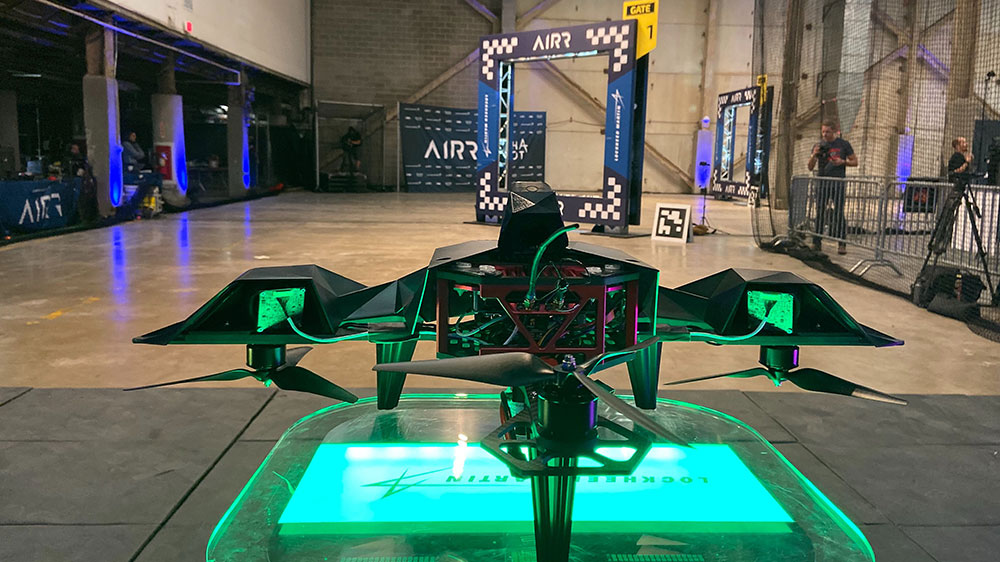
\includegraphics[width=0.80\textwidth]{imagenes/foehnAlphaPilot}
	\caption{Cuadricóptero empleado en el AlphaPilot 2019, mirando hacia la primera puerta del circuito \cite{foehn2020alphapilot}}
	\label{}
\end{figure}


Actualmente, el rendimiento obtenido por los drones de carreras autónomos aún está lejos de alcanzar el de los pilotos humanos. Es por esto que el afán por superar el nivel de los pilotos humanos es una motivación para los grupos de investigación por todo el mundo. El desarrollo de drones autónomos es un campo de estudio exigente que involucra el desarrollo de la tecnología existente en diversos campos de la robótica como: la estimación, el control, la generación de trayectorias o la percepción, entre otros. 

\section{Motivación}

El desarrollo de un sistema capaz de recorrer un circuito de forma autónoma sin interacción externa con cierta incertidumbre sobre el entorno, es un problema apasionante debido a las elevadas velocidades de vuelo y la limitada capacidad computacional, que exigen tener algoritmos de percepción y de estimación de estado más precisos y rápidos, así como algoritmos de planificación y de control más rápidos y ligeros, que permitan realizar cálculos a tiempo real.

Los avances obtenidos en diversos campos de la robótica durante el desarrollo de estos drones autónomos de carreras se pueden extrapolar para mejorar el rendimiento de los drones autónomos empleados para realizar distintas tareas con una mayor relevancia como pueden ser la aplicaciones industriales o como aquellas relacionadas con la búsqueda y rescate.

Los últimos avances en las plataformas de simulación enfocadas al desarrollo de sistemas de control de drones autónomos, como el simulador fotorrealista FlightGoggles desarrollado por Guerra et al \cite{guerra2019flightgoggles} empleado durante las pruebas clasificatorias del AlhpaPilot 2019, permiten probar el rendimiento de un sistema autónomo de forma realista y segura.



\section{Objetivos}
El objetivo propuesto consiste en diseñar la arquitectura de un sistema modular capaz de controlar un cuadrirrotor a través de un circuito de carreras de forma autónoma.

Debido a la gran complejidad que presenta el desarrollo completo de todos los módulos que intervienen en un dron de carreras autónomo, se han simplificado el desarrollo de los módulos de estimación de estado y de percepción del circuito, empleando datos provistos por el simulador. Es por esto que el trabajo se ha centrado en el desarrollo de la arquitectura del sistema y en el desarrollo de los módulos de control y generación de trayectorias, los cuales deben ser capaces de generar y seguir trayectorias agresivas a lo largo de todo el circuito a altas velocidades y con incertidumbre sobre el recorrido en sí.

Para el algoritmo de control se han implementado dos controladores del estado del arte, un controlador para orientaciones del aeronave con ángulos pequeños y otro para grandes ángulos y se ha comparado el rendimiento de ambos en el seguimiento de diversas trayectorias.

En cuanto a la generación de trayectorias, se ha optado por generar trayectorias polinómicas óptimas de tipo \textit{spline}. Para poder mejorar la capacidad de reacción del aeronave ante cambios en el circuito se ha dividido la generación de trayectorias en dos partes: la generación de una trayectoria completa a través de todo el circuito (largo plazo) y la generación de una trayectoria corta entorno a un horizonte temporal próximo a la posición del aeronave (corto plazo).

Para desarrollar los algoritmos y comparar el rendimiento del sistema realizado, se ha utilizado el simulador FlightGoogles, el cual fue empleado para las pruebas clasificatorias del AlphaPilot 2019 como entorno de pruebas.


%Este sistema estará formado por 3 partes principales:
%\begin{itemize}
%	\item \textbf{Estimación de estado:} Para poder recorrer el circuito es necesario tener una estimación precisa del estado de la aeronave a lo largo del tiempo. Para poder localizar el desarrollo de los 2 bloques posteriores se empleará la estimación provista por el simulador.
%	\item \textbf{}
%	\item \textbf{Generación de trayectorias:}
%\end{itemize}

Para poder llevar a cabo el desarrollo del trabajo de forma adecuada es conveniente desgranar los objetivos principales en tareas de alcance más reducido:

\begin{itemize}
	\item \textbf{Modulo de control}	
	\begin{itemize}
		\item Modelado dinámico del comportamiento de un cuadricóptero.
		\item Estudio del estado del arte acerca de los algoritmos de control más relevantes en las carreras de drones.
		\item Desarrollo teórico de los algoritmos de control para ángulos pequeños ($\phi,\theta  < \pi/6$) y para ángulos grandes ($\phi,\theta  \ge \pi/6 $) .
		\item Implementación de ambos algoritmos dentro del módulo de control.
		\item Ajuste de los parámetros de los controladores.
		\item Evaluación del rendimiento de ambos controladores en un entorno simulado.
				
	\end{itemize}

	\item \textbf{Generación de trayectorias}	
	\begin{itemize}
		\item Estudio del estado del arte acerca de los métodos de generación de trayectorias más empleados.
		\item Desarrollo teórico de los algoritmos de generación de trayectorias que se van a emplear.
		\item División del módulo generador de trayectorias en corto y largo plazo.
		\item Implementación de los algoritmos de generación de trayectorias empleados.
		\item Evaluación del rendimiento de los generadores de trayectorias mediante el recorrido del circuito de carreras en simulación.
	\end{itemize}

	\item \textbf{Arquitectura del sistema}	
	\begin{itemize}
		\item Estudio de las arquitecturas empleadas por los ganadores de las diversas competiciones de drones autónomos.
		\item Descomposición del sistema en los distintos módulos separados que compondrán la arquitectura final.
		\item Implementación de los módulos de estimación y percepción partiendo de las mediciones provistas por el simulador.
		\item Evaluación del funcionamiento completo de la arquitectura mediante el recorrido del circuito simulado. 
		
	\end{itemize}
	
	
\end{itemize}
	\chapter{Estado del arte}

Para contextualizar el trabajo desarrollado dentro del campo de las carreras de drones autónomos es necesario conocer los avances obtenidos por la comunidad robótica. Debido a que los contenidos del trabajo se han enfocado, principalmente, en torno al controlador y a la generación de trayectorias se ha profundizado en el estado del arte de estos campos enfocados a los drones de carreras. Adicionalmente, debido al objetivo del trabajo de generar un sistema coordinado, también se ha revisado el trabajo realizado por los finalistas de las carreras de drones autónomos más importantes.

\section{Control y generación de trayectorias}

En la primera década de los 2000, la mayoría del trabajo realizado con multirrotores empleaba controladores linealizados en torno al punto de equilibrio (\textit{hover}), los cuales, unicamente garantizan la estabilidad de la aeronave para pequeños ángulos de \textit{pitch} y \textit{roll} \cite{hoffmann2008quadrotor}. En cuanto a las trayectorias generadas, la mayoría de ellas son trayectorias polinómicas del tipo \textit{spline}, generadas interpolando una función entorno a los puntos de paso deseados \cite{vanek2005}\cite{barrientos2009}.

En 2008 V. Raffo et al. \cite{MPCRaffo2008} emplearon una estructura de control basada en un controlador predictivo basado en el modelo (MPC) que se encargaba de seguir la trayectoria y un controlador $\mathcal{H}_\infty$ que controlaba la rotación de la aeronave. Con esta estructura son capaces de seguir trayectorias sencillas de forma robusta ante perturbaciones.

En 2010, Guillula et al. \cite{gillula2010design} diseñaron un controlador capaz de realizar maniobras acrobáticas, como una voltereta hacia atrás, con un cuadricóptero de forma segura. Para ello emplearon un \textit{framework} para el diseño de regiones de cambio seguras, en las que cada región presenta un modelo dinámico distinto. Sin embargo, estas maniobras se generan de forma discontinua, necesitando analizar cada parte de la trayectoria de forma independiente y generar situaciones de cambio entre estos modos de forma segura. 

En 2011, Mellinger et al. \cite{MinimunSnap2011} presentan un controlador para cuadricópteros que permite realizar maniobras agresivas en un espacio tridimensional de forma continua. Este controlador no está linealizado en torno a ningún punto de funcionamiento, por lo que permite seguir trayectorias agresivas con un bajo error de seguimiento aunque el aeronave tenga ángulos grandes de \textit{roll} y \textit{pitch}. Este es uno de los controladores más usados actualmente debido al rendimiento que consigue con un algoritmo sencillo y con un bajo coste computacional.

En 2012, Mallikarjunan et al. \cite{mallikarjunan2012l1} diseñaron un controlador de actitud adaptativo, aplicando control $\mathcal{L}_1$, capaz de seguir trayectorias de forma precisa y robusta, con presencia de incertidumbres en el modelo de la aeronave y de las perturbaciones del entorno.

En 2016, Kamel et al. \cite{KamelMPC2016} comparan el rendimiento de dos MPCs, uno lineal y uno no lineal, en el seguimiento de trayectorias agresivas con un cuadricóptero. En estos experimentos observaron que, aunque ambos controladores eran capaces de seguir las trayectorias de forma satisfactoria, el controlador no lineal, conseguía un rendimiento ligeramente superior.

En 2017, Faessler et al. \cite{Faessler17ral} emplearon control LQR considerando tanto la dinámica del cuadricóptero, como la dinámica aislada de cada rotor. Además, consideran los limites de los rotores para priorizar la saturación de aquellas entradas que son relevantes para la estabilización del cuadricóptero. Asimismo, en 2018 \cite{Faessler18ral}, refinaron el controllador de Mellinger et al. considerando el arrastre (\textit{drag}) de los rotores dentro del modelo dinámico del cuadricóptero, en lugar de considerarlo como una perturbación externa desconocida, consiguiendo una ligera mejora en el seguimiento de trayectorias a alta velocidad.
 
En 2018, Falanga et al. \cite{falanga2018pampc} presentan un controlador MPC consciente de la percepción, el cual unifica el control y la planificación para satisfacer objetivos de acción y percepción de forma simultánea. Las trayectorias generadas por el MPC deben tener en cuenta ambos objetivos, para conseguir realizar maniobras complicadas mientras maximizan la visibilidad de puntos de interés por la aeronave.


\section{Carreras de drones autónomos}
Ganaron la competición IROS 2018 Autonomous Drone Race \cite{BeautyAndTheBeast}.

Recientemente \cite{foehn2020alphapilot}





	\chapter{Fundamentos teóricos}

	\chapter{Hardware}

	\chapter{Software}
	\chapter{Metodología}
	
\tb{En los capítulos anteriores se ha presentado los distintos algoritmos de control y generación de trayectorias que se emplearñan para conseguir recorrer un circuito con un \tb{dron} de carreras autónomo }. En este apartado se presenta la metodología empleada para superar las pruebas clasificatorias del Alphapilot 2019 

\section{Sistemas de referencia}


\section{Generación de \textit{waypoints}}
Para recorrer el circuito de forma satisfactoria es necesario que la aeronave atraviese las distintas puertas o \textit{gates} que componen el circuito en un orden concreto. Para conseguir esto es necesario conocer las posiciones de las puertas en el mundo y generar los puntos de paso necesarios para que la aeronave pase a través de ellas sin colisionar.

En la competición se proporciona el orden en el que se deben atravesar las puertas y una posición aproximada de las posiciones de cada una de ellas en el mundo. 

\begin{figure}[htb!]
	\centering
	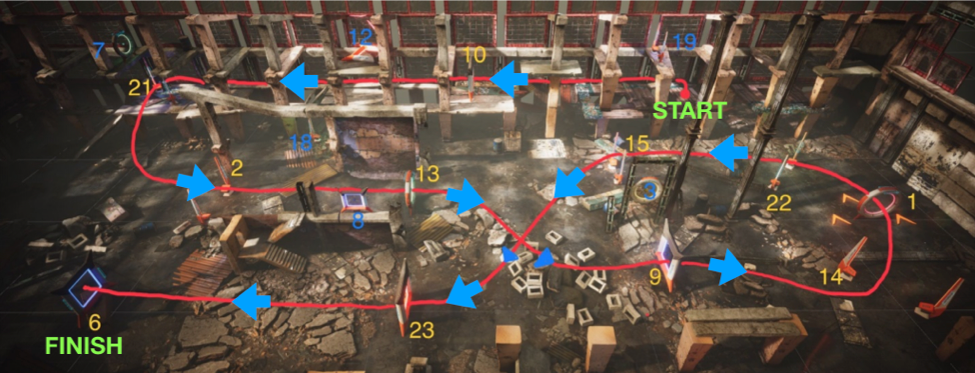
\includegraphics[width=\textwidth]{imagenes/diagramacircuito}
	\caption{Vista aérea del circuito en el simulador FightGoggles, las puertas que se deben traspasar se simbolizan con su número en color amarillo.}
	\label{waypoints:circuito}
\end{figure}

Como se puede observar en la figura \ref{waypoints:circuito} la aeronave debe recorrer 11 puertas, cada una con un número de identificación, en el orden indicado. 








\section{Trayectorias a largo y corto plazo}


	\chapter{Experimentos}

\begin{figure}[htb!]
	\centering
	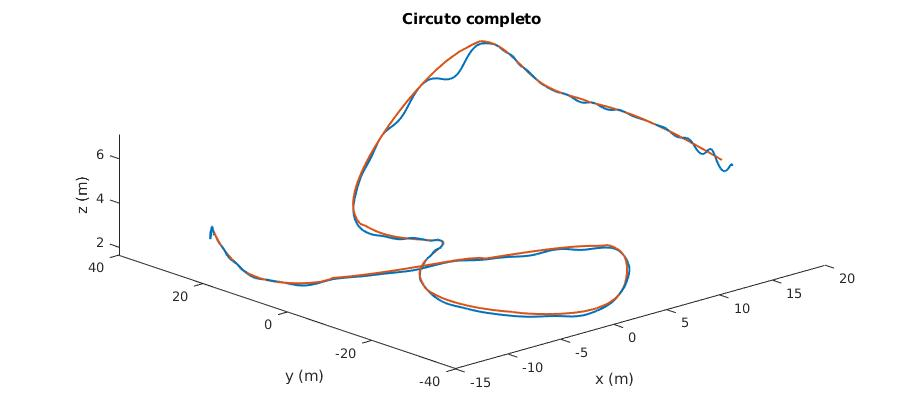
\includegraphics[width=\textwidth]{imagenes/circuitFigure}
	\caption{}
	\label{exp1:1}
\end{figure}

\begin{figure}[htb!]
	\centering
	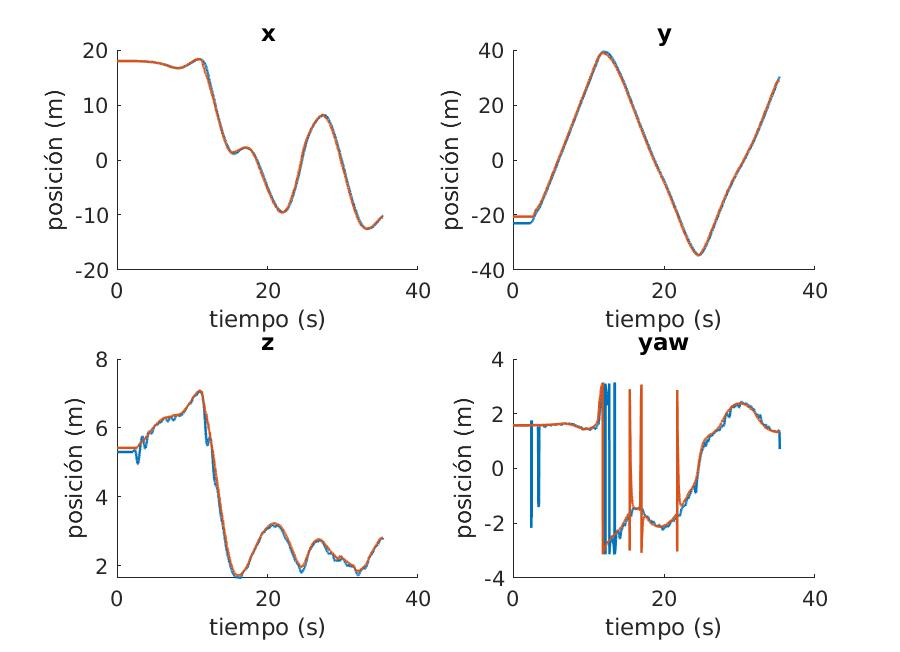
\includegraphics[width=\textwidth]{imagenes/positionFigure}
	\caption{}
	\label{exp1:2}
\end{figure}

\begin{figure}[htb!]
	\centering
	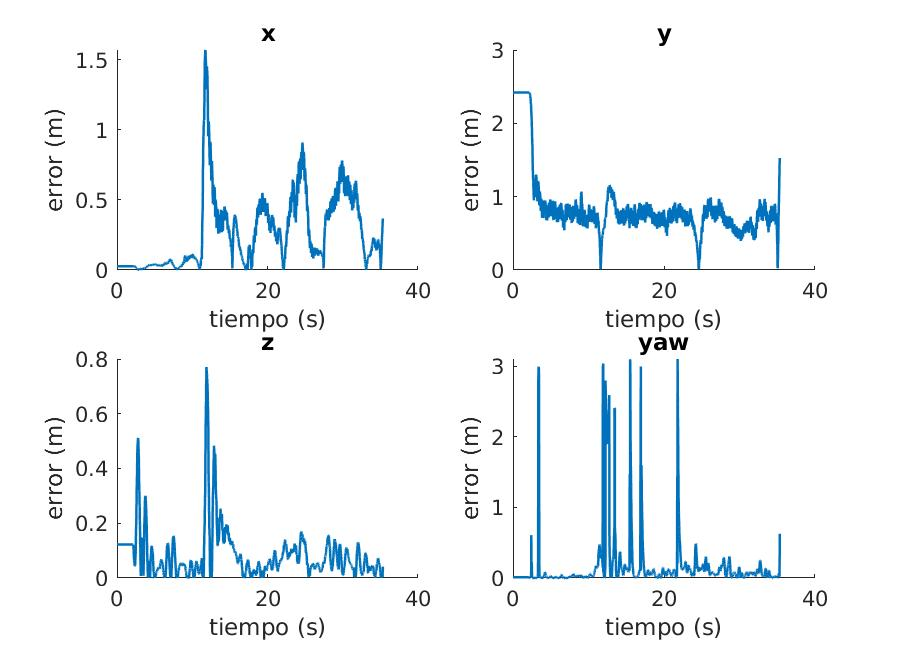
\includegraphics[width=\textwidth]{imagenes/errorFigure}
	\caption{}
	\label{exp1:3}
\end{figure}

\begin{table}[htb!]
	\centering

\begin{tabular}{l|c|c|c|}
	$\empty$&Eje x&Eje y&Eje z\\
\midrule
	Error máximo (m)&1.5685&1.1577&0.7707\\
	Error medio (m) &0.3143&0.7306&0.0796\\
	
\end{tabular}
\caption{Errores de seguimiento durante el recorrido del circuito.}
\end{table}

\section{Experimentos en simulación}
\section{Experimentos en real}
	%\chapter{Discusión}


	\chapter{Conclusiones y trabajo futuro}

\section{Conclusiones}

Durante el transcurso de este trabajo se ha desarrollado la arquitectura modular para un cuadricóptero de carreras autónomo. Esta modularidad de la arquitectura ha facilitado el desarrollo de los algoritmos de forma aislada así como el desarrollo de los experimentos de control, en los que se ha podido intercambiar los módulos de generación de trayectorias por módulos más sencillos de forma ágil. Esta modularidad también permitiría sustituir el módulo del simulador por un módulo de interfaz con una plataforma real, lo que facilitaría la realización de experimentos en real.

En cuanto al control del cuadricóptero se han conseguido implementar dos controladores del estado del arte de forma satisfactoria adaptándolos a las señales de control requeridas por el cuadricóptero. El empleo de herramientas como el \textit{dynamic reconfigure} de ROS han permitido realizar el ajuste de las ganancias de los controladores \textit{online}, lo que ha reducido considerablemente los tiempos necesarios para realizar estos ajustes.

Por otro lado, la decisión de separar la generación de trayectorias en dos partes, una a largo plazo y otra a largo plazo, ha permitido generar trayectorias de control óptimas en \textit{snap} con una alta reactividad frente a los cambios en las estimaciones de las puertas, manteniendo un bajo coste computacional en la generación de ambas trayectorias.

Finalmente, se han validado los desarrollos e implementaciones realizados en un entorno de simulación fotorrealista, consiguiendo completar el circuito de carreras completo de forma satisfactoria con una velocidad máxima de vuelo de 10,5 m/s en un tiempo inferior a los 23 segundos, lo que se situaría dentro de los mejores obtenidos el año pasado durante las clasificatorias virtuales del AlphaPilot2019.



\section{Trabajo futuro}

El trabajo realizado deja una arquitectura modular que permite su ampliación con nuevos módulos para adecuarla a la realización de distintas tareas de forma sencilla. Para una utilización del sistema en un caso real sería necesario implementar los módulos de estimación y percepción del entorno de una forma integral, empleando únicamente las medidas obtenidas por los sensores de la aeronave. 

Para mejorar el comportamiento del controlador sería conveniente emplear un controlador predictivo basado en el modelo (MPC), que permitiría reducir el error de seguimiento suavizando las acciones bruscas realizadas por el controlador cuando sufre cambios en la trayectoria de referencia. Junto con este controlador, se podrían emplear algoritmos de auto-identificación que permitan estimar \textit{online} el valor de los parámetros dinámicos de la aeronave, así como identificar posibles perturbaciones presentes en el entorno como podría ser el viento.

Finalmente, se podrían implementar métodos de optimización para calcular trayectorias que tengan en cuenta restricciones espaciales, lo que permitiría su empleo en entornos complicados con obstáculos alrededor. 












	\appendix
 
\chapter{Presupuesto y Planificación}

\section{Presupuesto}

El presupuesto del trabajo se puede separar en dos partes: recursos humanos y amortización de los equipos utilizados.

En cuanto a los recursos humanos empleados, se ha tenido una dedicación por parte del alumno de unas 400 horas, lo que se corresponde dentro del número de horas de dedicación esperadas en la realización de un Trabajo fin de Máster (12 ECTS). Un salario mensual de ayudante investigador a jornada completa en la universidad, es de unos 1250 euros, lo que se traduce en un coste de unos 8,33 euros la hora. El salario del tutor se ha extraído del portal de transparencia de la UPM. La dedicación del tutor ha sido de unas 30 horas de implicación en el trabajo.

\begin{figure}[htb!]
		\centering
		\begin{tabular}{|l|r|r|r|}
		\hline
		%\textbf{Recursos humanos} &Coste unitario [EUR] &Unidades&Total [EUR]\\
		
		\textbf{Recursos humanos} & Horas &Coste Horario [EUR]&Total [EUR]\\
		\hline
		
		Alumno & 400 & 8.33 &  3332 \\
		Tutor & 30& 33.72 & 1011.6 \\
		\hline
		\textbf{Total} & &  & \textbf{4343.6}\\
		\hline
		\end{tabular}\\
	
\end{figure}


En cuanto a la amortización del equipo, se ha empleado un ordenador para el desarrollo del software y para la realización de los experimentos. Se ha considerado una amortización lineal del 10 \% de la vida útil (4 años).

\begin{figure}[htb!]
	\centering
	\begin{tabular}{|l|r|r|r|}
		\hline
		\textbf{Equipo} & Precio &Coste Amortización(10\%)\\
		\hline
		Pc sobremesa & 1980 & 198\\
		\hline
		\textbf{Total} & & \textbf{198}\\
		\hline
\end{tabular}\\
\end{figure}

Con lo que el coste total del proyecto ha sido:

\begin{figure}[htb!]
	\centering
	\begin{tabular}{|l|r|r|r|}
		\hline
		\textbf{Concepto} &Total [EUR]\\
		\hline
		Recursos humanos & 4343.6\\
		Amortización del equipo & 198\\
		
		\hline
		\textbf{Total}   & \textbf{4541.6}\\
		\hline
	\end{tabular}\\
\end{figure}




\newpage
\section{Planificación}
La realización de este trabajo ha empleado un ritmo continuo de horas de trabajo desde su comienzo, a comienzos de abril. La dedicación media invertida en el desarrolo del trabajo ha sido de unas 35 horas semanales, durante un periodo de unos 3 meses, lo que da un total de unas 400 horas. El trabajo se ha realizado dentro del grupo de investigación CVAR (\textit{Computer Vision and Aerial Robotics}) del departamento de Electrónica Automática e Informática industrial de la Escuela Técnica Superior de Ingenieros Industriales (ETSII) perteneciente a la Universidad Politécnica de Madrid (UPM).

En cuanto a la distribución del trabajo en este tiempo, el trabajo comenzó a realizarse a finales de abril de 2020, durante el primer mes se realizó el curso sobre robótica aérea de UPenn, en la plataforma \textit{online} Coursera. La duración del curso se extendió hasta finales de abril. En mayo el trabajo se focalizó en el desarrollo de la arquitectura que se emplearía posteriormente, así como en el estudio del arte de los diferentes algoritmos de control y métodos de generación de trayectorias relevantes en el campo a estudiar. En junio y julio, se realizaron las implementaciones de los distintos algoritmos y se realizaron los primeros experimentos. Finalmente se ha redactado la memoria del proyecto en el mes de Septiembre. Se ha realizado un diagrama GANTT (\cref{gantt}) en el que se ha detallado más en profundidad la distribución temporal de las tareas. Asimismo, se ha esquematizado la organización del proyecto en un diagrama EDP 


\begin{figure}[htb!]
	\centering
	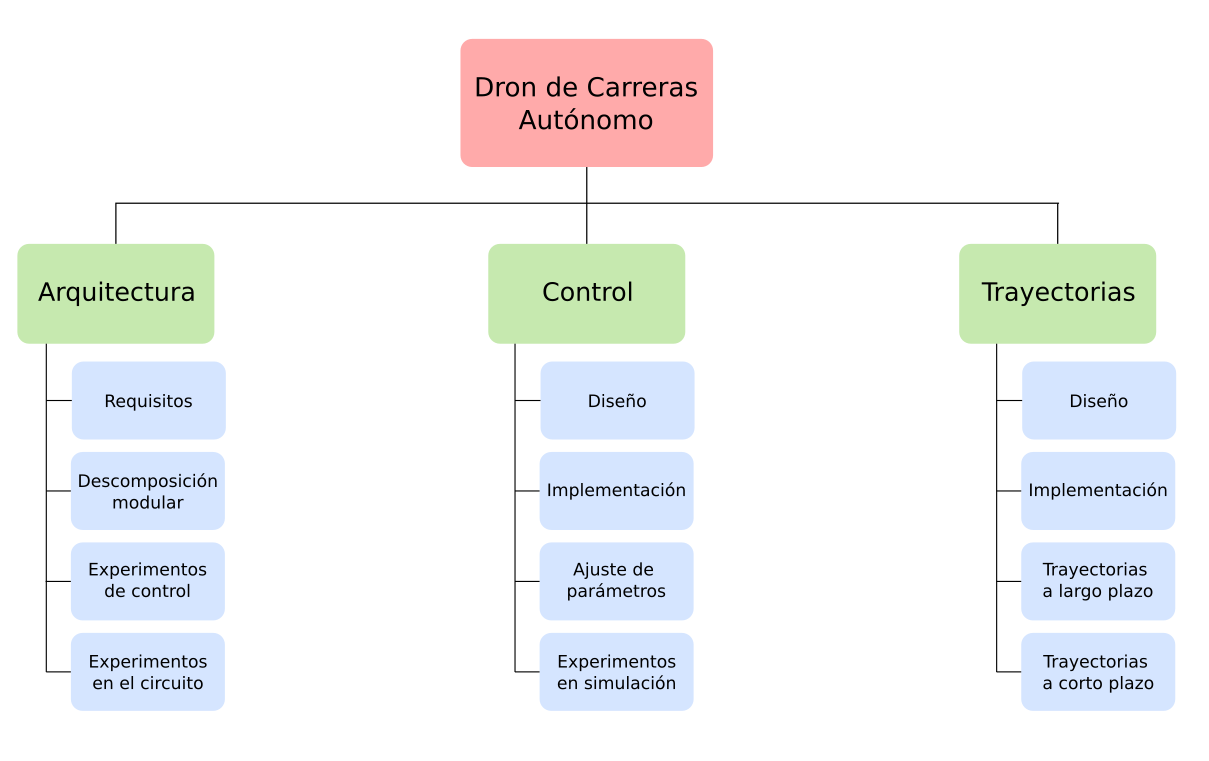
\includegraphics[width=0.85\textwidth]{imagenes/EDP}
	\caption{Diagrama EDP}
	\label{edp}
\end{figure}

\newpage

\textcolor{white}{aligment}
\begin{figure}[htb!]
	\centering
	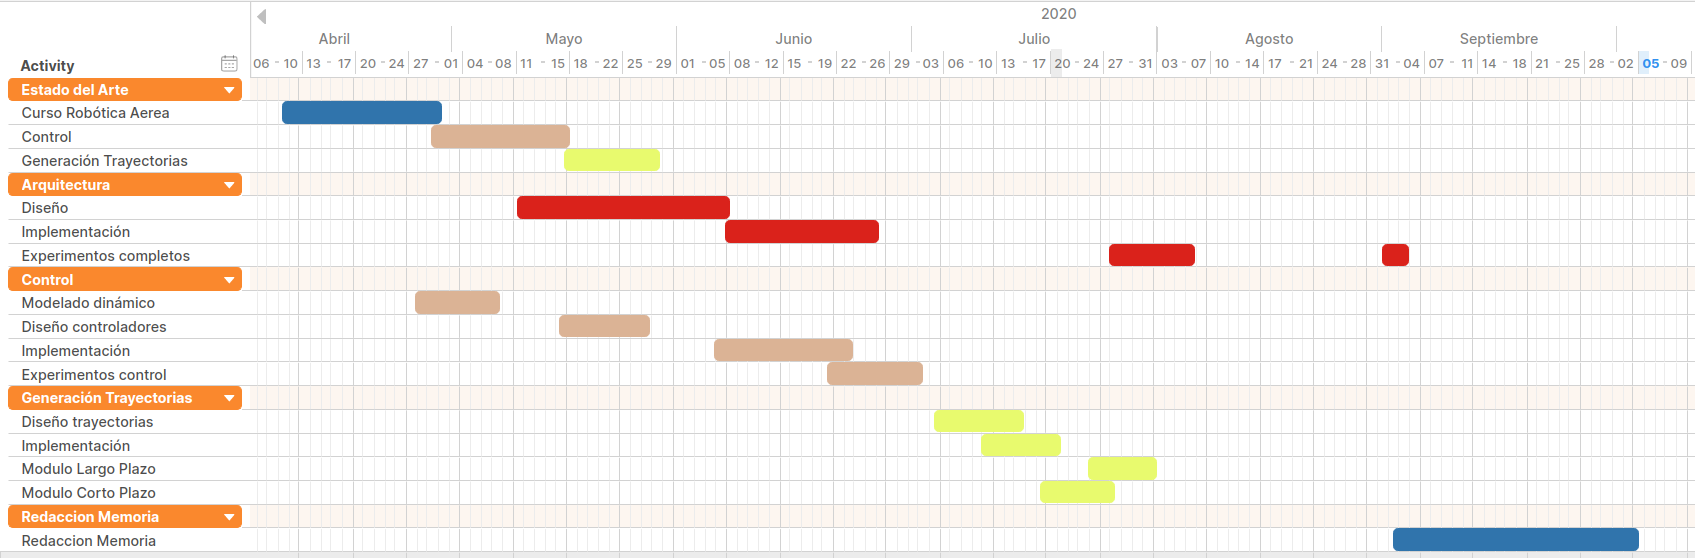
\includegraphics[angle=90,width =0.45\textwidth]{imagenes/gantt}
	\caption{Diagrama Gantt}
	\label{gantt}
\end{figure}


	
%	\pagenumbering{arabic}
%	
	\newpage
	\listoffigures
		\nocite{*}
	\bibliographystyle{bibliografia/IEEEtran}
	\bibliography{bibliografia/IEEEabrv,bibliografia/workBibliography}
	
\end{document}
